\title{Singular Values}
\subtitle{\SubTitleName}
\institute[]{\Course}
\author{\Instructor}
\maketitle   


\frame{\frametitle{Topics and Objectives}
\Emph{Topics} \\
%\TopicStatement
\begin{itemize}

    \item singular values of a matrix
    \item the connection between linear transforms, constrained optimization, and singular values 
    % \item the Singular Value Decomposition (SVD) and some of its applications

\end{itemize}

\vspace{0.5cm}

\Emph{Learning Objectives}\\

%\LearningObjectiveStatement

\begin{itemize}

    \item compute the singular values of a matrix
    \item interpret the singular values of a matrix in terms of a constrained optimization problem related to linear transforms
    % \item Compute the SVD for a rectangular matrix
    % \item Apply the SVD to 
    % \begin{itemize} 
    %     \item estimate the rank and condition number of a matrix, 
    %     \item construct a basis for the four fundamental spaces of a matrix, and
    %     \item construct a spectral decomposition of a matrix.
    % \end{itemize}
\end{itemize}

} 






\begin{frame}\frametitle{Singular Values}


    \begin{center}\begin{tikzpicture} \node [mybox](box){\begin{minipage}{0.62\textwidth}\vspace{4pt}
    
        The singular values of any $m\times n$ real matrix $A$ are the square roots of the eigenvalues of $A^TA$. 
        
    \end{minipage}};\node[fancytitle, right=10pt] at (box.north west) {\textbf{Definition}};\end{tikzpicture}\end{center}
    
    \vspace{6pt}
    
    \pause
    
    \onslide<2->{\Emph{Questions}}
    \begin{itemize}
        \item<2-> How might this definition connect to some of the other topics we covered? 
        \item<3-> How might singular values be viewed from a more geometric perspective? 
        \item<4-> Can the eigenvalues of $A^TA$ be negative? 
        \item<5-> What problems can singular values be used to solve? 
    \end{itemize}
    
    \vspace{12pt}
    \onslide<6->{These questions are explored throughout this presentation. }
    
\end{frame}



\begin{frame} \frametitle{Linear Transforms on the Unit Circle}

    \pause 
    The linear transform whose standard matrix is $$A = \frac{1}{\sqrt{2}}\spalignmat{1 -1;1 1}\spalignmat{2\sqrt{2} 0;0 \sqrt{2}} = \spalignmat{2 -1;2 1}$$ \pause transforms unit vectors in $\mathbb R^2$ to an ellipse, as shown below. 
    \pause 
    \vspace{-12pt}
    
    \begin{columns}
        \begin{column}{.1\textwidth}
        \end{column}
        \begin{column}{.3\textwidth}
        \begin{center}
            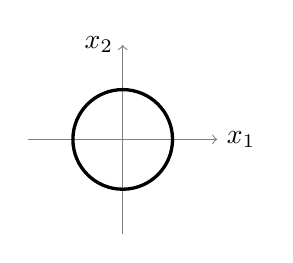
\begin{tikzpicture}[scale=0.6]
                \draw[->,gray] (-2,0) -- (2,0) node[right,black] {$x_1$};
                \draw[->,gray] (0,-2) -- (0,2) node[left,black] {$x_2$};
                \draw [rotate=0,black,very thick] (0,0) ellipse (30pt and 30pt);  
            \end{tikzpicture}
        \end{center}
        \end{column}        
        \begin{column}{.2\textwidth}
        \vspace{1cm}
        \begin{center}
            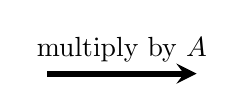
\begin{tikzpicture}[scale=0.95]
                \draw[->,thick,>=stealth,line width=0.75mm] (-3,0) -- node[above] {multiply by $A$} ++ (2,0);
            \end{tikzpicture}
        \end{center}
        \end{column}     
        \begin{column}{.3\textwidth}
        \begin{center}
            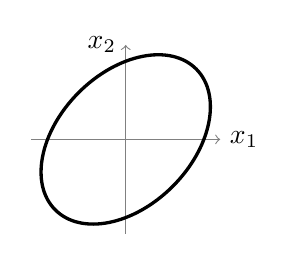
\begin{tikzpicture}[scale=0.6]
                \draw[->,gray] (-2,0) -- (2,0) node[right,black] {$x_1$};
                \draw[->,gray] (0,-2) -- (0,2) node[left,black] {$x_2$};
                \draw [rotate=45,black,very thick] (0,0) ellipse (60pt and 40pt);  
            \end{tikzpicture}
        \end{center}
        \end{column}       
        \begin{column}{.1\textwidth}
        \end{column}        
    \end{columns}
    
    \vspace{6pt}
    \pause \begin{center}
        What unit vector, $\vec v$, maximizes $||A \vec v||$? What is $||A \vec v||$ equal to? 
    \end{center}
\end{frame}



\begin{frame} \frametitle{Solution}

    Our goal is to maximize $\lVert A\vec v \rVert$ subject to $\lVert \vec v \rVert = 1$, in other words, 
    $$\max_{\lVert \vec v \rVert = 1}\lVert A\vec v \rVert$$
    \pause But the maximum occurs at the same location as $\lVert A\vec v \rVert^2$. 
    \begin{align*}
        \lVert A\vec v \rVert^2 = \vec v\,^T A^TA \vec v
    \end{align*}
    \pause
    $A^TA$ is symmetric.
    
    \pause 
    \vspace{12pt}
    \textit{We can answer some our questions with the eigenvalues of $A^TA$. }
\end{frame}



\begin{frame} \frametitle{Solution}
    We need the eigenvalues of $A^TA$. 
    \begin{align*}
        A^TA  = \spalignmat{2 2;-1 1}\spalignmat{2 -1;2 1} = \spalignmat{8 0;0 2} \quad \Rightarrow \quad \lambda = 8, 2
    \end{align*}
    Thus, 
    $$\max_{\lVert \vec v \rVert = 1}\lVert A\vec v \rVert^2 = 8$$
    So
    $$\max_{\lVert \vec v \rVert = 1}\lVert A\vec v \rVert = \sqrt8$$
    Thus, $\sqrt8$ is the maximum value that we were seeking. 
    
    \vspace{12pt}
    
    Next: what is the $\vec v$ that corresponds to this maximum? 

\end{frame}



\begin{frame} \frametitle{Solution}
    The unit eigenvector corresponding to the largest eigenvalue is the vector, $\vec v_1$, that maximizes $\lVert A\vec v \rVert$. 
    
    $$A^TA - \lambda I = \spalignmat{0 0;0 -6} \quad \Rightarrow \quad \vec v_1 = \spalignmat{1;0}$$
    
    The unit vector that maximizes $\lVert A\vec v \rVert$ is $\vec v_1 = \spalignmat{1;0}$.
\end{frame}



\begin{frame} \frametitle{Solution}    
    Recall that $A$ is the standard matrix for a transform that rotates and scales.
    
    $$A = \frac{1}{\sqrt{2}}\spalignmat{1 -1;1 1}\spalignmat{2\sqrt{2} 0;0 \sqrt{2}} = \spalignmat{2 -1;2 1}$$
    \vspace{-18pt}
        \begin{columns}
        \begin{column}{.1\textwidth}
        \end{column}
        \begin{column}{.3\textwidth}
        \begin{center}
            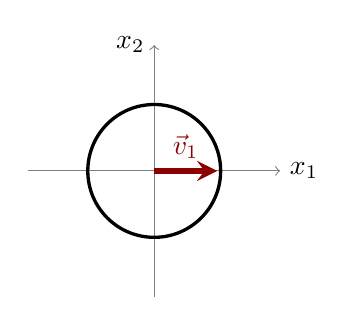
\begin{tikzpicture}[scale=0.8]
                \draw[->,gray] (-2,0) -- (2,0) node[right,black] {$x_1$};
                \draw[->,gray] (0,-2) -- (0,2) node[left,black] {$x_2$};
                \draw [rotate=0,black,very thick] (0,0) ellipse (30pt and 30pt);  
                \draw[->,thick,>=stealth,DarkRed,line width=0.75mm] (0,0) -- node[above] {$\vec v_1$} ++ (1,0);
            \end{tikzpicture}
        \end{center}
        \end{column}        
        \begin{column}{.2\textwidth}
        \vspace{1cm}
        \begin{center}
            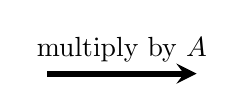
\begin{tikzpicture}[scale=0.95]
                \draw[->,thick,>=stealth,line width=0.75mm] (-3,0) -- node[above] {multiply by $A$} ++ (2,0);
            \end{tikzpicture}
        \end{center}
        \end{column}     
        \begin{column}{.3\textwidth}
        \begin{center}
            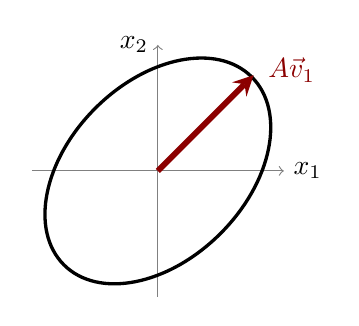
\begin{tikzpicture}[scale=0.8]
                \draw[->,gray] (-2,0) -- (2,0) node[right,black] {$x_1$};
                \draw[->,gray] (0,-2) -- (0,2) node[left,black] {$x_2$};
                \draw [rotate=45,black,very thick] (0,0) ellipse (60pt and 40pt);  
                \draw[->,thick,>=stealth,DarkRed,line width=0.75mm] (0,0) -- (1.52,1.52);
                \draw[DarkRed] (1.6,1.6) node[right] {$A\vec v_1$} ;
            \end{tikzpicture}
        \end{center}
        \end{column}       
        \begin{column}{.1\textwidth}
        \end{column}        
    \end{columns}
    \begin{center}
            The length of $A\vec v_1$ is the square root of the largest eigenvalue of $A^TA$, or $\sqrt 8$.
    \end{center}    
\end{frame}


\begin{frame} \frametitle{The Smallest Eigenvalue}    
    A similar process yields that the smallest eigenvalue of $A^TA$ is
    
    $$ \min_{\lVert \vec v \rVert = 1}\lVert A\vec v \rVert = \sqrt{2}, \quad \vec v_2 = \spalignmat{0;1}$$
    
    \pause
    

    \vspace{-6pt}
        \begin{columns}
        \begin{column}{.1\textwidth}
        \end{column}
        \begin{column}{.3\textwidth}
        \begin{center}
            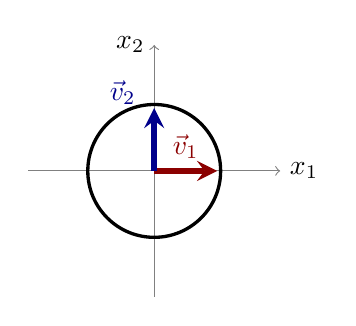
\begin{tikzpicture}[scale=0.8]
                \draw[->,gray] (-2,0) -- (2,0) node[right,black] {$x_1$};
                \draw[->,gray] (0,-2) -- (0,2) node[left,black] {$x_2$};
                \draw [rotate=0,black,very thick] (0,0) ellipse (30pt and 30pt);  
                \draw[->,thick,>=stealth,DarkRed,line width=0.75mm] (0,0) -- node[above] {$\vec v_1$} ++ (1,0);
                \draw[->,thick,>=stealth,DarkBlue,line width=0.75mm] (0,0) -- ++ (0,1);
                \draw[DarkBlue] (-.5,0.9) node[above] {$\vec v_2$} ;
            \end{tikzpicture}
        \end{center}
        \end{column}        
        \begin{column}{.2\textwidth}
        \vspace{1cm}
        \begin{center}
            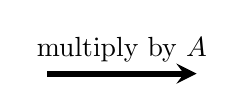
\begin{tikzpicture}[scale=0.95]
                \draw[->,thick,>=stealth,line width=0.75mm] (-3,0) -- node[above] {multiply by $A$} ++ (2,0);
            \end{tikzpicture}
        \end{center}
        \end{column}     
        \begin{column}{.3\textwidth}
        \begin{center}
            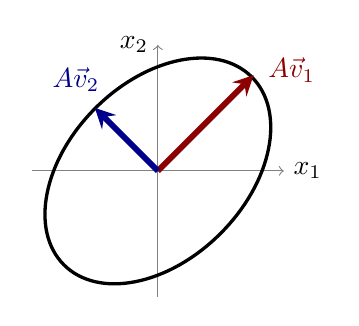
\begin{tikzpicture}[scale=0.8]
                \draw[->,gray] (-2,0) -- (2,0) node[right,black] {$x_1$};
                \draw[->,gray] (0,-2) -- (0,2) node[left,black] {$x_2$};
                \draw [rotate=45,black,very thick] (0,0) ellipse (60pt and 40pt);  
                \draw[->,thick,>=stealth,DarkRed,line width=0.75mm] (0,0) -- (1.52,1.52);
                \draw[->,thick,>=stealth,DarkBlue,line width=0.75mm] (0,0) -- (-1.,1.);                
                \draw[DarkRed] (1.6,1.6) node[right] {$A\vec v_1$} ;
                \draw[DarkBlue] (-1.3,1.1) node[above] {$A\vec v_2$} ;
            \end{tikzpicture}
        \end{center}
        \end{column}       
        \begin{column}{.1\textwidth}
        \end{column}        
    \end{columns}
    \begin{center}
    \pause 
            $\lVert A\vec v_2 \rVert$ is the square root of the smallest eigenvalue of $A^TA$, which is $\sqrt 2$.
            
         
    \end{center}    
\end{frame}


\begin{frame} \frametitle{Singular Values are the Eigenvalues of $A^TA$}    

    Let $\sigma_1 = \sqrt{\lambda_1} = \sqrt{8}$, and $\sigma_2 = \sqrt{\lambda_2}= \sqrt{2}$. 
    
    \vspace{-6pt}
        \begin{columns}
        \begin{column}{.1\textwidth}
        \end{column}
        \begin{column}{.3\textwidth}
        \begin{center}
            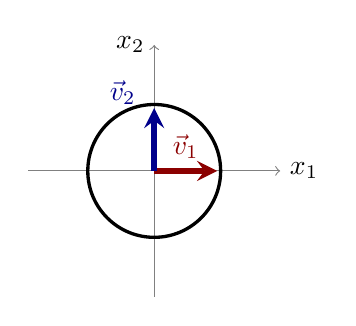
\begin{tikzpicture}[scale=0.8]
                \draw[->,gray] (-2,0) -- (2,0) node[right,black] {$x_1$};
                \draw[->,gray] (0,-2) -- (0,2) node[left,black] {$x_2$};
                \draw [rotate=0,black,very thick] (0,0) ellipse (30pt and 30pt);  
                \draw[->,thick,>=stealth,DarkRed,line width=0.75mm] (0,0) -- node[above] {$\vec v_1$} ++ (1,0);
                \draw[->,thick,>=stealth,DarkBlue,line width=0.75mm] (0,0) -- ++ (0,1);
                \draw[DarkBlue] (-0.5,0.9) node[above] {$\vec v_2$} ;
            \end{tikzpicture}
        \end{center}
        \end{column}        
        \begin{column}{.2\textwidth}
        \vspace{1cm}
        \begin{center}
            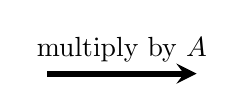
\begin{tikzpicture}[scale=0.95]
                \draw[->,thick,>=stealth,line width=0.75mm] (-3,0) -- node[above] {multiply by $A$} ++ (2,0);
            \end{tikzpicture}
        \end{center}
        \end{column}     
        \begin{column}{.3\textwidth}
        \begin{center}
            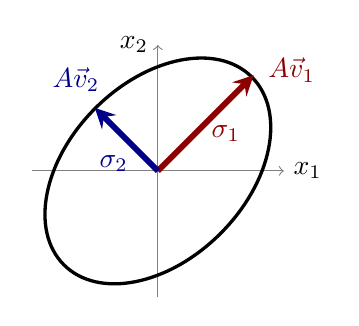
\begin{tikzpicture}[scale=0.8]
                \draw[->,gray] (-2,0) -- (2,0) node[right,black] {$x_1$};
                \draw[->,gray] (0,-2) -- (0,2) node[left,black] {$x_2$};
                \draw [rotate=45,black,very thick] (0,0) ellipse (60pt and 40pt);  
                \draw[->,thick,>=stealth,DarkRed,line width=0.75mm] (0,0) -- (1.52,1.52);
                \draw[->,thick,>=stealth,DarkBlue,line width=0.75mm] (0,0) -- (-1.,1.);                
                \draw[DarkRed] (1.6,1.6) node[right] {$A\vec v_1$} ;
                \draw[DarkBlue] (-1.3,1.1) node[above] {$A\vec v_2$} ;
                
                \onslide<2->{\draw[DarkRed] (0.7,0.6) node[right] {$\sigma_1$} ;}
                \onslide<3->{\draw[DarkBlue] (-0.7,-0.16) node[above] {$\sigma_2$} ; }              
            \end{tikzpicture}
        \end{center}
        \end{column}       
        \begin{column}{.1\textwidth}
        \end{column}        
    \end{columns}
    \begin{center}
    \onslide<4->{In other words: the length of $A\vec v_i$ is the square root of the eigenvalues of $A^TA$, or $\sqrt{\lambda_i}$.}
    \end{center}    
\end{frame}








\begin{frame}\frametitle{Eigenvalues of $A^TA$ Are Non-Negative}

    \vspace{-12pt}

    \begin{center}\begin{tikzpicture} \node [mybox](box){\begin{minipage}{0.55\textwidth}\vspace{4pt}
    
        The eigenvalues of $ A ^{T} A $ are non-negative. 
        
    \end{minipage}};\node[fancytitle, right=10pt] at (box.north west) {\textbf{Theorem}};\end{tikzpicture}\end{center}
    
    \vspace{6pt}
    
    \pause
    
    \Emph{Proof}: recall that $\vec v_j^T\vec v_j = \vec v_j\cdot\vec v_j = \lVert \vec v_j \rVert ^2 =1$ because $\vec v_j$ are \Emph{unit} eigenvectors of $A^TA$.  
    \pause 
    \begin{align*}
        \lVert A \vec v_j\rVert ^2 =
        (A \vec v_j) ^{T} A \vec v_j= \vec v_j A^T A \vec v_j = \lambda _j \vec v_j ^T \vec v_j = \lambda _j \geq 0. 
    \end{align*}
    \pause 
    Therefore: \pause
    \begin{itemize}
        \item the eigenvalues of $A^TA$ must be real and non-negative
        \item the singular values of $A$, which are the square roots of the eigenvalues, must also be real and non-negative
    \end{itemize} 
    


\end{frame}









% \begin{frame}\frametitle{Singular Values}
    
%     % The matrix $ A ^{T} A $ is always symmetric, with non-negative eigenvalues $ \lambda _1 \geq \lambda _2 \geq \cdots \geq \lambda _n \geq 0$.  Let $ \{\vec v_1 ,\dotsc, \vec v_n\}$ be the associated orthonormal eigenvectors.  

%     % \vspace{12pt} 
    
%     Earlier in this presentation we saw that the largest singular value of $A$ is:\pause the maximum length of $A\vec v$ subject to $\lVert \vec v \rVert =1$. \pause
    
%     $$\sigma_1 = \max_{\lVert \vec v \rVert = 1}\lVert A\vec v \rVert$$
    
%     \vspace{12pt}
%     \pause 
%     What about the other singular values? 
% \end{frame}


% \begin{frame}\frametitle{Singular Values}    
%     \begin{itemize}
%         \item Recall that the second largest eigenvalue of a symmetric matrix gives the maximum of $\lVert A\vec v \rVert$ subject to $$ \lVert \vec v \rVert =1 , \quad \vec v \cdot \vec u_1 = 0$$
%         \item The second largest eigenvalue is $\sigma_2$
%         \item Thus, $\sigma_2$ 
%     \end{itemize}
%     Likewise with the remaining eigenvalues. 
% \end{frame}






\begin{frame}\frametitle{Note: Singular Values are Ordered}

    %  The matrix $ A ^{T} A $ is always symmetric, with non-negative eigenvalues $ \lambda _1 \geq \lambda _2 \geq \cdots \geq \lambda _n \geq 0$. 
    Because the eigenvalues of $A^TA$ are non-negative, the singular values of $A$ must also be real and non-negative. \pause They can be ordered from largest to smallest. 
    
    \pause 

    \begin{center}\begin{tikzpicture} \node [mybox](box){\begin{minipage}{0.95\textwidth}\vspace{4pt}
    
        The singular values, $\sigma_j$, of any $m\times n$ real matrix $A$ are the square roots of the eigenvalues of $A^TA$. Singular values are arranged in decreasing order.
        
        $$\sigma _1 = \sqrt {\lambda _1 } \geq \sigma _2 = \sqrt {\lambda _2}  \geq \ \cdots \ \geq \sigma _n=\sqrt {\lambda _n} $$ 
        
    \end{minipage}};\node[fancytitle, right=10pt] at (box.north west) {\textbf{Definition}};\end{tikzpicture}\end{center}
    
    \vspace{6pt}
    This is a standard convention for singular values. 
    
    
    
    
\end{frame}


\begin{frame}\frametitle{Singular Values are Lengths}

    It also follows from the previous slide that the singular values of $A$ represent lengths of vectors in $\mathbb R^n$. That is, when showing that the eigenvalues of $A^TA$ are non-negative, we saw that
    \onslide<2->{ $$|| A\vec v_i||^2 = \lambda_i $$}
    \onslide<3->{ Therefore, $$|| A\vec v_i||= \sigma_i $$}
    \onslide<4->{We make use of this relationship when constructing the SVD of a matrix. }
\end{frame}







\frame{\frametitle{Summary}

    \SummaryLine \vspace{4pt}
    \begin{itemize}\setlength{\itemsep}{8pt}

        \item the singular values of any $m\times n$ real matrix $A$ are the square roots of the eigenvalues of $A^TA$
        \item singular values are related to the lengths of $\lVert A \vec x \rVert$ for $\lVert \vec x \rVert = 1$
        \item singular values are real and non-negative
        \item singular values are arranged in decreasing order

    \end{itemize}
    
    \vspace{6pt}
}
